\documentclass[10pt]{article}

\usepackage[a4paper, margin=2cm]{geometry}
\usepackage{amsmath,amssymb,amsthm}
\usepackage{booktabs}
\usepackage{array}
\usepackage{hyperref}
\usepackage[numbers,super,sort&compress]{natbib}
\usepackage{xcolor}
\usepackage{graphicx}

\hypersetup{colorlinks=true, linkcolor=blue!50!black, citecolor=blue!50!black, urlcolor=blue!50!black}

\newtheorem{theorem}{Theorem}
\newtheorem{proposition}[theorem]{Proposition}
\newtheorem{corollary}[theorem]{Corollary}
\theoremstyle{definition}
\newtheorem{definition}[theorem]{Definition}
\theoremstyle{remark}
\newtheorem{remark}[theorem]{Remark}

\setlength{\parskip}{4pt}
\setlength{\parindent}{12pt}

\title{\textbf{Scalar Rewards Cannot Fully Represent Pluralistic LLM Preferences
}\\[0.3em]
\large Hodge residuals and Condorcet diagnostics reveal projection loss\\ in language-model alignment data}


\author{Anonymous Author(s)}
\date{}

\begin{document}

\maketitle

\vspace{-2em}

\begin{abstract}
\noindent
Modern large language model alignment converts heterogeneous human judgements into scalar rewards, rankings, or constitutions. This conversion is operationally necessary for RLHF, DPO, and related post-training methods, but it assumes that local pairwise preferences can be projected onto a single global ordering without losing structure. Social choice theory shows why this assumption can fail: aggregate preferences may contain cycles even when the underlying judgements are meaningful. Here we develop a social-choice diagnostic for measuring this failure in LLM preference data. We represent pairwise feedback as an edge flow over alternatives and decompose it into a scalar, reward-representable component and a cyclic residual. We first apply the diagnostic to PRISM, a dataset of human ratings of 21 language models. The pooled PRISM tournament is mostly scalarisable: raw cycle counts are null-like ($p=0.326$), while the weighted cyclic residual is modestly above a fitted transitive null ($\rho_{\mathrm{cyc}}=0.0422$ versus null mean $0.0365$; $p=0.0446$). We then analyze MultiPref, an LLM-native preference dataset with normal and expert annotators and aspect labels. MultiPref exposes no prompt-local three-model agendas, so prompt-local Condorcet cycles are not identifiable; its pooled six-model source tournament is directionally transitive but has aspect-dependent scalar projection residuals above a support-preserving transitive null. Finally, we use Moral Machine to examine moral pluralism under two constructions. Direct country-level tournaments over 20 character types contain rare cycles, but cycle rates, parity-obstruction rates, and scalar projection residuals are not elevated above a participant-shuffling null (cycle-fraction $p=0.652$; residual $p=0.960$). A model-based latent moral-profile construction, by contrast, produces larger cycle and parity deviations from its null. Together these results show that scalar rewards are useful projections, not complete representations, of pluralistic human feedback. The residual left by scalar projection is precisely the component that standard scalar reward learning cannot represent, and it should be measured with support audits and null models rather than silently collapsed into one global reward.
\end{abstract}

\section*{}
\vspace{-1em}

\section*{Introduction}

The central problem in contemporary alignment is no longer only whether a language model follows instructions, but whose preferences those instructions and rewards are meant to represent. Reinforcement learning from human feedback\cite{ouyang2022,stiennon2020}, direct preference optimisation\cite{rafailov2023}, constitutional approaches\cite{bai2022}, and ranking-based reward modelling all transform many local human judgements into a scalar object: a reward, a ranking, or a policy preference. This scalar object is then used as if it were a coherent representation of what the relevant population wants from an LLM.

That assumption is stronger than it first appears. A scalar reward does not merely summarise data; it imposes a transitive geometry on the data. If output $a$ is scored above output $b$, and $b$ above $c$, then the same scalar score must place $a$ above $c$. This is what makes optimisation possible. It is also what makes scalar alignment lossy when the empirical preference relation contains cyclic structure: $a$ is preferred to $b$, $b$ to $c$, and $c$ to $a$. Such structure cannot be represented by any real-valued reward, regardless of model size, optimiser, or training procedure.

Social choice theory has studied this obstruction for decades. When many individuals each hold coherent preferences, the collective relation produced by majority voting can still cycle. Condorcet cycles\cite{black1948}, Arrow's theorem, Sen's liberal paradox, and related results show that preference aggregation can fail under reasonable desiderata\cite{arrow1951,sen1970}. Topological versions of these impossibility results sharpen the point: continuous aggregation respecting anonymity and unanimity exists only under restrictive conditions on the preference space\cite{chichilnisky1980,chichilnisky1983,baryshnikov1993}. For LLM alignment, the question is not whether these impossibilities exist in the abstract, but whether they leave measurable structure in the datasets used to train and evaluate aligned systems.

We answer this empirically by measuring scalar projection loss. Pairwise feedback defines a skew-symmetric edge flow on a graph or complex whose vertices are alternatives: model outputs, language models, or moral profiles. A scalar reward induces a gradient edge flow, because each edge is explained by the difference between two scores. Following Hodge-theoretic ranking\cite{jiang2011}, we project the empirical edge flow onto the closest scalar gradient field and measure the residual. This residual is not ordinary prediction error. It is the part of the preference relation that no scalar reward can represent.

The paper is organised around LLM alignment first. Our primary case study is PRISM\cite{kirk2024}, a human-feedback dataset in which approximately 1,500 participants rate responses from 21 language models. PRISM is an appropriate test bed because it is directly about subjective and multicultural LLM alignment, and because its opening-turn design yields pairwise model comparisons under shared prompts. We find that PRISM is mostly scalarisable: roughly 96\% of the weighted edge-flow energy is captured by the best scalar ranking. The remaining component is small but detectable under the fitted transitive null. Raw Condorcet cycle counts are null-like, while the weighted cyclic residual lies just above the null 95th percentile. The lesson is precise: current LLM preference data may look rankable at the level of winners and losers while still containing a measurable non-gradient component that scalar reward models must discard.

We then test the same diagnostic on MultiPref\cite{miranda2025}, a preference-tuning dataset containing stable source-model identifiers, persistent evaluator IDs, normal and expert annotations, and separate overall, helpfulness, truthfulness, and harmlessness labels. MultiPref is an important negative-control case. It does not expose prompt-local Condorcet tests: after auditing both prompt identifiers and literal prompt text, no prompt group contains all three pairwise edges needed for a three-model tournament. Its global six-model tournament is dense and acyclic in every pooled normal/expert aspect aggregate, reflecting a strong and unsurprising model-quality ordering. Yet the pairwise margins are not perfectly additive: scalar residuals are small for overall and helpfulness but larger for truthfulness and harmlessness, and most exceed a calibrated transitive null on the observed model-pair support. MultiPref therefore scopes the claim: not all LLM preference data exhibit Condorcet cycles, but even clean model-quality rankings can contain calibrated projection loss in their margin geometry.

We then turn to Moral Machine\cite{awad2018} as a case where moral pluralism is explicit rather than embedded in LLM ratings. Here the object being aggregated matters. A direct margin-preserving construction over 20 character-type alternatives contains rare country-level cycles, but its cycle and residual rates are explained by a participant-shuffling null. A latent moral-profile construction asks a different, more pluralism-facing question: if respondents are represented by scalar weights over moral dimensions and majority rule aggregates them over synthetic moral profiles, do collective cycles appear? Under that construction, cycle and parity diagnostics are elevated relative to the same kind of null. Moral Machine therefore supplies a construction-sensitive lesson: explicit moral content does not automatically imply excess aggregate intransitivity, but pluralistic aggregation over morally meaningful alternatives can instantiate scalar-ordering obstructions.

Our contribution is not the claim that human preferences are chaotic, nor that scalar rewards should be abandoned. The claim is narrower and more useful for alignment: scalar reward learning is a projection of pluralistic preference data, and the projection can lose structured information. Since there are impossibility results for aggregating human preferences, there are corresponding preference structures that LLMs cannot faithfully represent under scalar post-training objectives. Alignment systems should therefore report Condorcet-aware diagnostics and treat high-residual regions as candidates for personalisation, deliberation, or multi-objective decision rules rather than treating one global reward as the complete representation of pluralism.

\section{A topological diagnostic for scalar reward misfit}
\label{sec:framework}

\subsection{Scalar rankings as global orientations}

Let $\mathcal{A} = \{a_1, \ldots, a_K\}$ be a set of alternatives. A scalar reward or ranking is a function $r : \mathcal{A} \to \mathbb{R}$. It induces a pairwise relation by score differences: $a_i \succ a_j$ if and only if $r_i > r_j$. Because real-valued $>$ is transitive, the induced relation is acyclic. Geometrically, $r$ is a global orientation of the complete graph on $\mathcal{A}$ by a potential function.

A pairwise comparison dataset, by contrast, gives only local information: for some pairs $(i, j)$, we observe a signed margin $W_{ij} \in \mathbb{R}$ with $W_{ji} = -W_{ij}$, indicating how much the population prefers $a_i$ to $a_j$. The empirical edge flow $W$ may or may not be globally orientable by a scalar $r$.

In LLM alignment, the alternatives may be candidate responses to a prompt, source models in a model-comparison tournament, or abstract response types. Standard reward modelling assumes that these local comparisons can be explained by score differences. The diagnostic below asks how much of the observed LLM preference field survives that scalar projection and how much is necessarily left as cyclic residual.

\subsection{Scalar rewards as exact preference gradients}

The scalar assumption has an equivalent edge-flow form. Fix an arbitrary orientation of the observed comparison graph and let $B$ be its edge--vertex incidence matrix, so that for an oriented edge $e=(i,j)$, $(Br)_e=r_i-r_j$. A scalar reward model therefore predicts an edge flow in the column space $\mathrm{im}(B)$. In a Bradley--Terry or logistic reward model this statement holds on the log-odds scale:
\begin{equation}
\ell_{ij}
\;=\;
\log\frac{P(a_i\succ a_j)}{P(a_j\succ a_i)}
\;=\;
r_i-r_j.
\label{eq:bt-logit}
\end{equation}
Thus scalar reward learning assumes that the empirical preference field is, up to statistical error, an exact discrete gradient.

\begin{theorem}[Exact-gradient criterion]\label{thm:exact-gradient}
Let $F$ be a skew-symmetric edge flow on a connected observed graph. There exists a scalar potential $r$ with $F_{ij}=r_i-r_j$ on every observed edge if and only if the circulation of $F$ around every cycle is zero:
\begin{equation}
\sum_{\ell=1}^{m} F_{v_\ell v_{\ell+1}} = 0,
\qquad v_{m+1}=v_1,
\end{equation}
for every closed walk $v_1,\ldots,v_m,v_1$ in the graph.
\end{theorem}
\begin{proof}
If $F_{ij}=r_i-r_j$, then summing around any closed walk telescopes:
\[
(r_{v_1}-r_{v_2})+(r_{v_2}-r_{v_3})+\cdots+(r_{v_m}-r_{v_1})=0.
\]
Conversely, assume all cycle circulations vanish. Fix a root vertex $v_0$. For any vertex $v$, choose a path $v_0=u_0,u_1,\ldots,u_m=v$ and define
\[
r_v=-\sum_{\ell=0}^{m-1} F_{u_\ell u_{\ell+1}} .
\]
This definition is path independent: two different paths from $v_0$ to $v$ form a closed walk, and the assumed zero circulation makes their sums equal. For an observed oriented edge $(i,j)$, take a path from $v_0$ to $j$ obtained by appending $(i,j)$ to a path from $v_0$ to $i$. Then $r_i-r_j=F_{ij}$. Hence $F$ is a gradient flow.
\end{proof}

The theorem is the finite-graph version of the obstruction we use throughout the paper. A scalar reward model is not merely a predictor of pairwise labels; it is a potential function whose induced logit field has zero circulation on every cycle. Nonzero circulation is therefore an exact algebraic certificate that some component of the observed pairwise field is not scalar-reward representable.

\subsection{Condorcet cycles as exact obstructions}

A directed triple $a_i \to a_j \to a_k \to a_i$ in the oriented edge flow is a Condorcet cycle. If $r$ represents the orientation, then $r_i > r_j$ and $r_j > r_k$ imply $r_i > r_k$, contradicting $r_k > r_i$. Hence:

\begin{proposition}[Cycle obstruction]\label{prop:cycle}
If the oriented relation induced by $W$ contains a Condorcet cycle, no scalar function $r$ represents $W$ exactly on those edges.
\end{proposition}
\begin{proof}
Suppose $a_i\to a_j\to a_k\to a_i$ is represented by a scalar $r$. Then $r_i>r_j$, $r_j>r_k$, and $r_k>r_i$. By transitivity of $>$ on $\mathbb{R}$, the first two inequalities imply $r_i>r_k$, contradicting $r_k>r_i$.
\end{proof}

This is a structural statement about an observed object. The presence of a single cycle already rules out exact scalar representation. It does not by itself say that the population preference field is genuinely cyclic rather than a finite-sample perturbation of a transitive one; that requires a separate null-model comparison.

Higher-order analogues can sharpen the diagnostic, but only relative to an explicit complex. Livson \emph{et al.}\cite{livson2026} show that Condorcet's paradox can be represented topologically as non-orientability in a constructed preference surface. In the finite tournament setting used here, we report the parity of the cycle indicator across the triangular faces of 4-subsets as a discrete obstruction statistic inspired by that framework. We do not infer literal manifold non-orientability unless the corresponding preference complex has been explicitly constructed.

\subsection{The cyclic residual: scalar projection loss}

Cycle counts ignore the size of pairwise margins. A signed edge flow $W$ with skew-symmetry $W_{ij} = -W_{ji}$ can be projected onto the subspace of gradient flows. Each ranking $r \in \mathbb{R}^K$ induces an edge flow $(\nabla r)_{ij} = r_i - r_j$; the best scalar ranking minimises weighted squared error:
\begin{equation}
r^\star \;=\; \arg\min_{r \in \mathbb{R}^K}\;\sum_{(i,j)\in E}\omega_{ij}\bigl(W_{ij} - (r_i - r_j)\bigr)^{2},
\label{eq:rstar}
\end{equation}
where $\omega_{ij}\geq 0$ is an edge support weight and $E$ is the set of observed pairs. The cyclic residual is $W_{\mathrm{cyc}} = W - \nabla r^\star$, and the cyclic residual mass is the fraction of weighted edge energy outside the gradient subspace:
\begin{equation}
\rho_{\mathrm{cyc}}(W) \;=\; \frac{\sum_{(i,j)\in E}\omega_{ij}\bigl(W_{ij}-(r^\star_i-r^\star_j)\bigr)^{2}}{\sum_{(i,j)\in E}\omega_{ij}W_{ij}^{2}}.
\label{eq:rho}
\end{equation}
This is the implementation-friendly form of the Hodge decomposition for ranking flows\cite{jiang2011}. Plainly, $\rho_{\mathrm{cyc}}$ is the share of the weighted preference signal that no scalar reward can explain. A value near $0$ indicates near-perfect scalar representability; values near $1$ indicate that scalar projection discards most of the signal.

\begin{proposition}[Energy decomposition]\label{prop:energy}
Let $\langle X,Y\rangle_{\omega}=\sum_{(i,j)\in E}\omega_{ij}X_{ij}Y_{ij}$ and $\|X\|_{\omega}^{2}=\langle X,X\rangle_{\omega}$. The solution $r^\star$ in Equation~\eqref{eq:rstar} is the weighted orthogonal projection of $W$ onto the gradient subspace. Consequently,
\begin{equation}
\|W\|_{\omega}^{2}
\;=\;
\|\nabla r^\star\|_{\omega}^{2}
\;+\;
\|W-\nabla r^\star\|_{\omega}^{2},
\label{eq:energy-decomposition}
\end{equation}
and
\begin{equation}
\rho_{\mathrm{cyc}}(W)
\;=\;
\min_{r}\frac{\|W-\nabla r\|_{\omega}^{2}}{\|W\|_{\omega}^{2}}
\;=\;
1-\frac{\|\nabla r^\star\|_{\omega}^{2}}{\|W\|_{\omega}^{2}} .
\label{eq:rho-energy}
\end{equation}
\end{proposition}
\begin{proof}
The set of all gradient flows $\{\nabla r:r\in\mathbb{R}^{K}\}$ is a linear subspace of the finite-dimensional edge-flow space equipped with the weighted inner product $\langle\cdot,\cdot\rangle_\omega$. Equation~\eqref{eq:rstar} is exactly the least-squares projection of $W$ onto this subspace. The normal equations imply that the residual $W-\nabla r^\star$ is orthogonal to every gradient flow, in particular to $\nabla r^\star$. The Pythagorean identity then gives Equation~\eqref{eq:energy-decomposition}, and dividing by $\|W\|_\omega^2$ gives Equation~\eqref{eq:rho-energy}.
\end{proof}

\begin{proposition}[Projection residual]\label{prop:residual}
Assume the denominator in Equation~\eqref{eq:rho} is positive. Then $\rho_{\mathrm{cyc}}(W)=0$ if and only if there exists a scalar $r$ such that $W_{ij}=r_i-r_j$ for every observed edge $(i,j)\in E$.
\end{proposition}
\begin{proof}
Equation~\eqref{eq:rstar} is the weighted least-squares projection of $W$ onto the linear subspace of gradient flows. The residual norm is zero exactly when $W$ lies in that subspace. This is equivalent to the existence of some scalar potential $r$ whose edge differences equal all observed margins.
\end{proof}

Proposition~\ref{prop:energy} gives the quantity its operational meaning. The numerator in Equation~\eqref{eq:rho} is not the error of a particular reward model; it is the minimum weighted squared distortion achieved by the best possible scalar reward on the observed graph. Thus $\rho_{\mathrm{cyc}}$ is a lower bound on the normalised squared distortion incurred by any scalar reward representation of the same edge margins.

\subsection{Pluralistic aggregation can create residual without individual irrationality}

The obstruction above does not require individual annotators to be irrational or internally inconsistent. Cyclic residual can arise from aggregating several coherent scalar perspectives.

\begin{proposition}[Coherent voters, cyclic aggregate]\label{prop:pluralism-cycle}
There exist three groups, each with a transitive scalar utility over three alternatives, whose equally weighted majority edge flow contains a directed 3-cycle and therefore is not exactly representable by any single scalar reward.
\end{proposition}
\begin{proof}
Let the alternatives be $A,B,C$. Consider three equally weighted groups with scalar utilities
\[
u_1(A)=2,\;u_1(B)=1,\;u_1(C)=0,
\]
\[
u_2(B)=2,\;u_2(C)=1,\;u_2(A)=0,
\]
and
\[
u_3(C)=2,\;u_3(A)=1,\;u_3(B)=0.
\]
Each group has a strict transitive ranking induced by a real-valued utility. Majority aggregation gives $A\succ B$ for groups 1 and 3, $B\succ C$ for groups 1 and 2, and $C\succ A$ for groups 2 and 3. Hence the aggregate orientation is $A\to B\to C\to A$. Equivalently, the signed majority margins satisfy $W_{AB}=W_{BC}=W_{CA}=1/3$, whose circulation around the triangle is $1$. By Theorem~\ref{thm:exact-gradient}, no scalar potential can represent this aggregate edge flow exactly.
\end{proof}

This example is deliberately minimal. In LLM preference data, the analogous mechanism can arise when annotators or subpopulations place different scalar weights on response features such as helpfulness, harmlessness, factuality, brevity, or tone. Each perspective may be scalar internally, while the aggregate edge flow over shared alternatives contains a non-gradient component.

\subsection{Operational non-orientability}

We use ``non-orientability'' cautiously and operationally. Directed Condorcet cycles obstruct exact scalar representation of the majority orientation (Proposition~\ref{prop:cycle}); a positive cyclic residual $\rho_{\mathrm{cyc}}>0$ quantifies scalar projection loss in the signed margins (Proposition~\ref{prop:residual}). These are diagnostic claims about observed finite objects. They are not, by themselves, claims that PRISM, MultiPref, or Moral Machine reconstructs a Klein bottle, projective plane, or any other literal non-orientable manifold. A manifold-orientability claim would require an explicit cycle-complex reconstruction and validation of the modelling assumptions used in the topological social-choice framework.

\section{Case study 1: PRISM reveals scalar projection loss in LLM preference aggregation}
\label{sec:prism}

The PRISM alignment dataset\cite{kirk2024} is our primary empirical case because it directly measures subjective preferences over large language model outputs. The dataset contains survey and conversation data from 1,500 participants, of whom 1,396 progressed to conversations with large language models. In each opening turn of a conversation, the participant writes a prompt and four randomly selected language models (out of a pool of 21) respond. The participant scores each of the four responses on a $1$--$100$ scale. Later turns continue with the highest-scoring model and present within-model A/B variants, and are excluded from the model-level analysis because they do not compare different source models. Each opening turn yields up to $\binom{4}{2}=6$ pairwise model comparisons under the same user and prompt, and aggregating across users and prompts yields an approximately complete 21-model tournament.

\subsection{Constructing the model-preference edge flow}

For score-difference threshold $\delta\geq 0$, the induced pairwise comparison from a conversation in which user $u$ scores models $i$ and $j$ is $+1$ if $s_{u}(i)-s_{u}(j)>\delta$, $-1$ if $s_{u}(j)-s_{u}(i)>\delta$, and a tie otherwise. We use $\delta=5$ throughout the main analysis, so that small score differences are treated as ties. We first average comparisons within each user across their conversations, and then average users equally to form a 21-by-21 skew-symmetric edge flow $W$ whose entries are user-weighted pairwise margins. Edges with fewer than $n_{\min}=25$ contributing users are excluded from the canonical graph, and the canonical orientation threshold is $\tau=0$.

After applying these settings, the pooled canonical analysis uses 7,828 valid opening-turn ballots and 42,306 user-weighted pairwise comparisons. All 21 models and all 210 unordered model-pair edges appear in the pooled graph.

\subsection{Cycles and cyclic residual against a transitive null}

We compute both diagnostics on the pooled edge flow: the Condorcet cycle rate among the $\binom{21}{3}=1{,}330$ eligible triples, and the cyclic residual $\rho_{\mathrm{cyc}}$ from Equation~\eqref{eq:rho}. To assess statistical significance, we fit a scalar Bradley--Terry-style edge model\cite{bradley1952} to the empirical margins and simulate synthetic tournaments under this transitive data-generating process while holding the observed edge supports and support weights fixed. With $B=5{,}000$ simulations we compute empirical $p$-values for both statistics.

\begin{figure}[t]
\centering
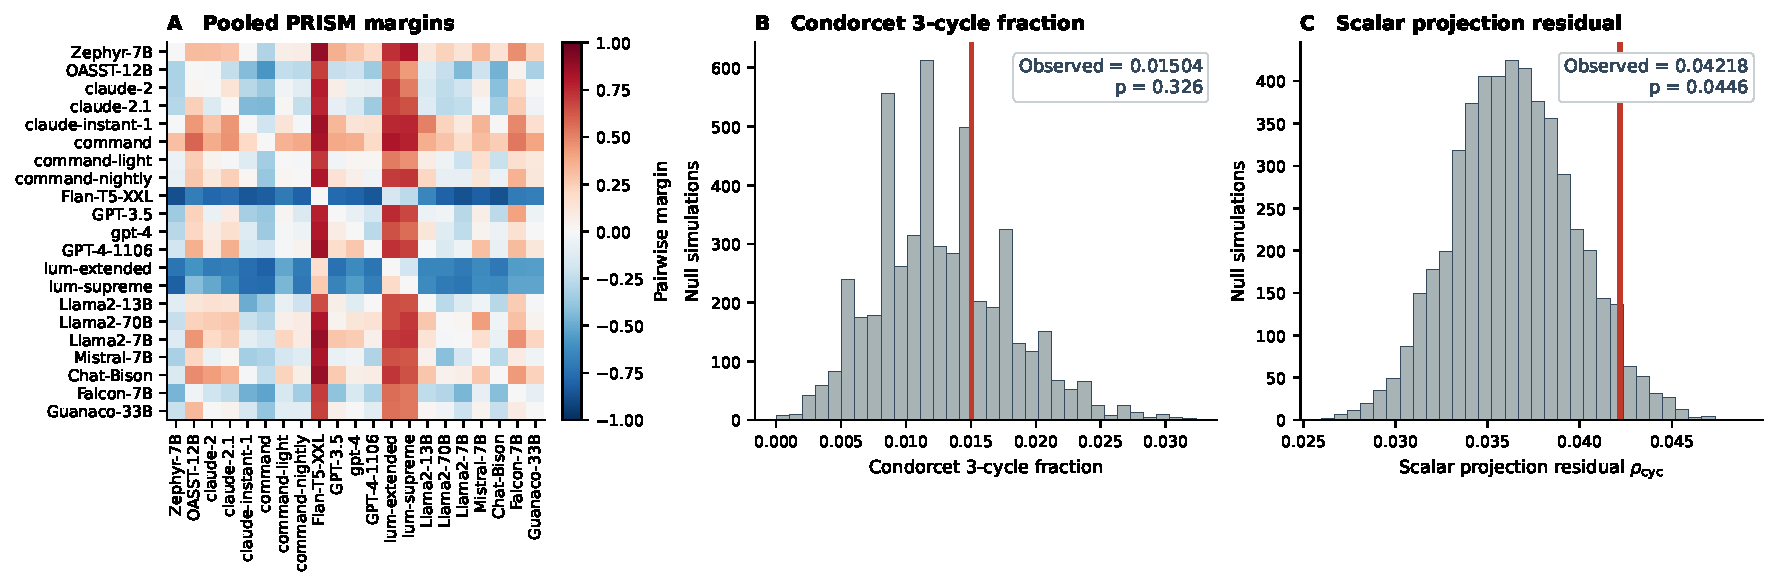
\includegraphics[width=\textwidth]{figures_generated/prism_results.pdf}
\caption{\textbf{PRISM model preferences are mostly scalar, with a small non-gradient residual.} The best scalar ranking explains approximately $95.8\%$ of the weighted edge-flow energy in the pooled 21-model tournament. Raw Condorcet cycle counts are consistent with a fitted transitive null, while the weighted cyclic residual is modestly larger than expected under the same null. Cycle counts and weighted residuals answer different questions and need not move together.}
\label{fig:prism}
\end{figure}

Figure~\ref{fig:prism}A shows the pooled signed margin matrix, with a visible dominant model-quality axis but also local departures from a perfectly additive ordering. Figure~\ref{fig:prism}B calibrates the qualitative Condorcet statistic against the fitted transitive null, while Figure~\ref{fig:prism}C performs the same calibration for the margin-aware scalar projection residual. The pooled 21-model tournament contains 20 cyclic triples among 1,330 eligible triples, a cycle rate of $\mathrm{CR}=0.0150$. The fitted transitive null produces a comparable mean cycle rate of $0.0128$ and the empirical $p$-value is $0.326$. Raw Condorcet cycle counting therefore detects no robust departure from transitivity in PRISM at the population level. The cyclic residual tells a different story. We measure $\rho_{\mathrm{cyc}}=0.0422$, against a null mean of $0.0365$ and a null 95th percentile of $0.0420$. The empirical $p$-value is $0.0446$ with $5{,}000$ simulations.

These two numbers together support a precise statement. The pooled PRISM tournament is mostly scalar: the best scalar ranking captures approximately $1-\rho_{\mathrm{cyc}}\approx 95.8\%$ of the weighted edge-flow energy. But the residual is not zero, and under the fitted edge-level transitive null it lies just above the 95th percentile. Raw cycle counting misses this signal because it ignores the size of pairwise margins; the cyclic residual detects it because it weights edges by their squared margin. Cycles and weighted residuals are answering different questions, and the right answer in PRISM is that the population edge flow has small but detectable non-gradient structure even when its cycle count is null-like.

\paragraph{Threshold sensitivity.} The observed residual magnitude is not driven by the canonical preprocessing thresholds. With $n_{\min}=25$, sweeping $\delta\in\{0,2,5,10\}$ gives $\rho_{\mathrm{cyc}}=0.0386,0.0406,0.0422,0.0427$. At the canonical $\delta=5$, sweeping $n_{\min}\in\{10,25,50,100\}$ gives $\rho_{\mathrm{cyc}}=0.0422,0.0422,0.0422,0.0399$; the first three thresholds retain all 210 unordered model-pair edges, and $n_{\min}=100$ retains 193. The orientation threshold $\tau$ affects the binary cycle count but not $\rho_{\mathrm{cyc}}$, which is computed from the signed margins before orientation. With $\tau=0$, cycle rates across $\delta=0,2,5,10$ are $0.0135,0.0143,0.0150,0.0120$; with $\tau\in\{0.05,0.10\}$, these weak-margin cycles disappear. Thus the observed residual is stable over the tested $\delta$ and $n_{\min}$ settings, but the null-calibrated PRISM excess remains modest and the binary cycle count is threshold-sensitive.

\subsection{Localisation: simple explanations do not hold}
\label{sec:localisation}

It is natural to look for the source of the residual in a single explanatory variable: stated values, choice-attribute salience, or demographic composition. None of these simple explanations holds.

\paragraph{Stated-preference clusters.} PRISM asks participants to rate the importance of eight stated values (creativity, diversity, factuality, fluency, helpfulness, personalisation, safety, values). A natural pluralistic-pooling hypothesis is that within-cluster preferences are internally scalar while pooling across clusters creates cycles, that is, $\rho_{\mathrm{cyc}}(W^{\mathrm{pooled}})>\sum_g \pi_g\rho_{\mathrm{cyc}}(W^{(g)})$. The observed pattern reversed this inequality. With $K=3$ clusters, the user-weighted mean within-cluster residual was $0.0927$ versus $0.0422$ pooled; with $K=5$ clusters, $0.1169$. Most cluster-specific residuals were not exceptional against cluster-specific transitive nulls. PRISM contains a dominant global model-quality axis that pooling actually stabilises; explicit stated-value clustering does not isolate internally scalarisable electorates.

\paragraph{Choice attributes.} PRISM records performance and choice attributes that explain why the highest-rated model was preferred. These are winner-conditioned, not per-model scores, and so cannot be used as direct safety or factuality ratings for losing models. High-attribute subsets showed descriptively larger cyclic residuals than the pooled tournament, but matched transitive nulls explained much of this through reduced edge support. Low-attribute subsets often had larger residuals than high-attribute ones. Choice attributes can localise edges and identify regions for follow-up, but they do not currently provide evidence that high value salience independently produces non-scalar structure.

\paragraph{Demographic strata.} Stratifying by English proficiency, marital status, age, education, and gender, several well-supported strata retained residuals above stratum-specific transitive-null baselines after $5{,}000$ simulations, including never-married users, native English speakers, university bachelor's-degree holders, married users, male users, and users aged $25$--$34$ (Table~\ref{tab:strata}). Raw cycle rates again did not provide the robust signal. These subgroup findings are exploratory: the strata are correlated, not pre-registered, and we report Benjamini--Hochberg false-discovery-rate $q$-values (Methods) rather than treating them as confirmatory. The right interpretation is that the estimated edge flow for some strata has more non-gradient mass than expected under a stratum-specific transitive null, not that any demographic group is intrinsically inconsistent.

\begin{table}[h]
\centering
\small
\begin{tabular}{@{}lrrrr@{}}
\toprule
\textbf{Tournament} & $\mathrm{CR}_{\mathrm{obs}}$ & $\mathrm{CR}_{\mathrm{null}}$ & $\rho_{\mathrm{cyc,\,obs}}$ & $p_{\rho}$ \\
\midrule
Pooled PRISM            & 0.0150 & 0.0128 & 0.0422 & $0.0446$ \\
Never married           & 0.0226 & 0.0236 & 0.0618 & $0.0022$ \\
Native speaker          & 0.0218 & 0.0196 & 0.0585 & $0.0044$ \\
University bachelor's   & 0.0286 & 0.0309 & 0.0811 & $0.0156$ \\
Married                 & 0.0455 & 0.0409 & 0.1150 & $0.0248$ \\
Male                    & 0.0180 & 0.0252 & 0.0702 & $0.0288$ \\
Age 25--34              & 0.0184 & 0.0344 & 0.0969 & $0.0492$ \\
\bottomrule
\end{tabular}
\caption{\textbf{Canonical PRISM tournaments against a fitted transitive null.} Canonical settings: $\delta=5$, $n_{\min}=25$, $\tau=0$. Raw cycle rates are generally not elevated above the null. The weighted cyclic residual mass $\rho_{\mathrm{cyc}}$ is the more sensitive signal, but the pooled excess is modest under the current fitted-null implementation. Subgroup rows are exploratory; we report Benjamini--Hochberg false-discovery-rate corrected $q$-values in Extended Data, and interpret them as aggregate edge-flow properties of group-level tournaments rather than individual-level claims.}
\label{tab:strata}
\end{table}

\section{Case study 2: MultiPref scopes the LLM-native claim}
\label{sec:multipref}

MultiPref\cite{miranda2025} is closer to post-training preference data than PRISM. It contains pairwise comparisons between responses generated by six source models, stable prompt and model identifiers, normal-worker and expert-worker annotations, persistent evaluator IDs, and separate preferences for overall quality, helpfulness, truthfulness, and harmlessness. We flatten the nested human annotations into 31,934 annotation rows from 10,461 raw comparisons. Preference labels are mapped to signed edge contributions with \texttt{clearly better}=1, \texttt{slightly better}=0.5, and ties contributing zero edge support.

The first result is a support audit. Prompt-local Condorcet tests require a full three-edge agenda for some prompt: model $A$ versus $B$, $B$ versus $C$, and $C$ versus $A$ under the same prompt. MultiPref does not provide this structure. After excluding same-model comparisons, 4,886 prompt groups have usable model-pair support. Of these, 2,331 contain one model-pair edge and 2,555 contain two; none contain three. Grouping by literal prompt text rather than \texttt{prompt\_id} gives the same result. Thus prompt-local Condorcet cycles are not identifiable in MultiPref.

The global model-source tournament is dense. All 15 unordered edges among the six models are observed, with 1,438--1,860 annotations per edge. The pooled, normal-worker, and expert-worker majority orientations are acyclic for every aspect: $0$ cyclic triples among the 20 possible triples in each group-aspect aggregate. This is not surprising. The overall and helpfulness relations largely follow a strong model-quality ordering in which newer or stronger source models defeat weaker ones.

The scalar residual nevertheless remains non-zero, and it is larger than expected under a calibrated transitive null that preserves the observed model-pair support and per-edge annotation weights. Figure~\ref{fig:multipref}A shows that the residual is small for overall quality and helpfulness but larger for truthfulness and harmlessness, while Figure~\ref{fig:multipref}B shows the dense pooled overall margin matrix whose majority orientation remains transitive. In the pooled tournament, $\rho_{\mathrm{cyc}}=0.0085$ for overall quality, $0.0097$ for helpfulness, $0.0417$ for truthfulness, and $0.0832$ for harmlessness, compared with null means $0.0018$, $0.0017$, $0.0105$, and $0.0403$, respectively. The one-sided empirical $p$-values are $p<0.001$ for overall, helpfulness, and truthfulness, and $p=0.0258$ for harmlessness; all four pooled tests survive Benjamini--Hochberg correction. Normal-worker and expert-worker residuals show the same pattern for overall, helpfulness, and truthfulness, whereas harmlessness is not elevated within either subgroup after calibration. The appropriate conclusion is therefore narrower than a Condorcet-cycle claim but stronger than a descriptive margin audit: MultiPref does not support prompt-local or aggregate Condorcet cyclicity, but it does show statistically calibrated, aspect-dependent margin geometry that is not exactly representable by one scalar score.

\clearpage

\begin{figure}[!htbp]
\centering
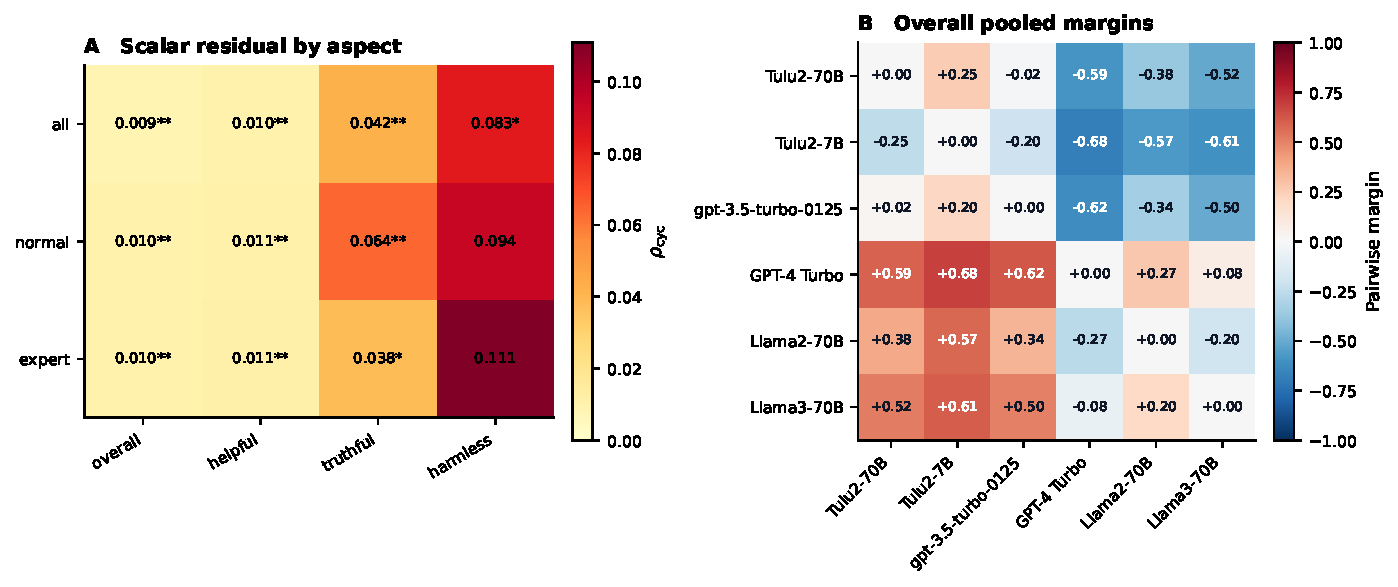
\includegraphics[width=\textwidth]{figures_generated/multipref_results.pdf}
\caption{\textbf{MultiPref is globally dense but prompt-locally too sparse for Condorcet-cycle identification.} The dataset supports a global source-model tournament over six models, but no prompt group contains a fully supported three-model agenda. Aggregated majority orientations are transitive in all reported group-aspect aggregates. A support-preserving transitive null shows that scalar projection residuals are nevertheless elevated for pooled overall, helpfulness, truthfulness, and harmlessness margins, with weaker subgroup evidence for harmlessness.}
\label{fig:multipref}
\end{figure}

\section{Case study 3: Moral Machine and construction-sensitive pluralism}
\label{sec:mm}

As a third case study, the Moral Machine experiment\cite{awad2018} collected approximately 40 million pairwise moral decisions from approximately 4 million participants across 233 countries. Each scenario asks the respondent to choose which group of characters an autonomous vehicle should spare in an unavoidable collision. The choices vary across character types and moral dimensions such as species, number of lives, age, lawfulness, social status, gender, fitness, and action versus inaction. The dataset is the canonical empirical example of a domain where collective moral judgement is expected to be heterogeneous across cultures.

\subsection{Direct character-type tournaments}

We first test whether collective moral judgement admits a single global ranking over the character types that appear in the experiment. For each respondent with at least eight valid scenarios, we estimate a signed preference vector over the 20 canonical Moral Machine character types by summing saved-side character counts and subtracting non-saved-side counts. For each country with at least 200 retained respondents, the pairwise majority across respondents defines a tournament over these 20 character-type alternatives. This direct margin-preserving construction retains 1,851,181 respondents and 105 country tournaments.

For each country tournament we compute four diagnostics: (i) the cycle fraction, defined as the proportion of the $\binom{20}{3}=1{,}140$ triples that form a Condorcet cycle; (ii) the odd-parity 4-subset fraction, defined as the proportion of $\binom{20}{4}=4{,}845$ 4-subsets whose cycle-indicator parity across the four triangular faces is odd; (iii) a country-level parity-obstruction indicator, taking value $1$ if at least one 4-subset has odd parity; and (iv) the scalar projection residual $\rho_{\mathrm{cyc}}$ computed from the signed majority margins. The parity statistic is a finite simplicial diagnostic motivated by topological social-choice theory; it is not, by itself, a proof that the empirical preference object is a literal non-orientable manifold.

We then compare this direct construction with a model-based latent moral-profile construction. The motivation is value pluralism and multidimensional social choice: moral disagreement can involve how people trade off several legitimate moral dimensions, and majority rule over multidimensional alternatives can cycle even when individuals are internally coherent scalar maximisers\cite{berlin1969,raz1986,plott1967,mckelvey1976}. Moral Machine itself varies dimensions such as species, number of lives, age, lawfulness, social status, gender, fitness, and action, and prior computational Moral Machine models represent choices as trade-offs over such abstract moral features\cite{awad2018,noothigattu2018,kim2018moral}. In our latent analysis, each respondent is represented by signed weights over moral dimensions. Synthetic moral profiles are represented as vectors in this moral-dimension space, and respondent $i$ ranks profile $m$ by $u_i(m)=\langle \beta_i,x_m\rangle$. Majority rule is then applied within countries over these profile alternatives. The construction is not intended as a unique representation of moral truth; it is a model-based stress test of how scalar projection loss changes when alternatives are represented at the level where pluralistic value trade-offs are expressed.

\subsection{Null model}

Any apparent cyclic structure could in principle reflect finite-sample noise, weak margins, or the baseline heterogeneity already present in the respondent-level preference vectors. We therefore compare aggregate rates against a participant-shuffling null. Holding each respondent's preference vector and each country's sample size fixed, we shuffle the country labels and recompute the country-level tournaments and their invariants. This null preserves individual preferences but destroys cross-cultural clustering. We use $n=500$ permutations and report standardised deviations $z=(\text{obs}-\text{null mean})/\text{null SD}$ together with empirical $p$-values.

The null does not decide whether an observed Condorcet cycle is an obstruction: a cycle in a finite majority relation is already not representable by a scalar ranking. The null only addresses the stronger enrichment question, namely whether cycles or residuals are more frequent than expected under the support, sample sizes, and respondent-level heterogeneity of the dataset.

\clearpage

\subsection{Results}

\begin{figure}[!htbp]
\centering
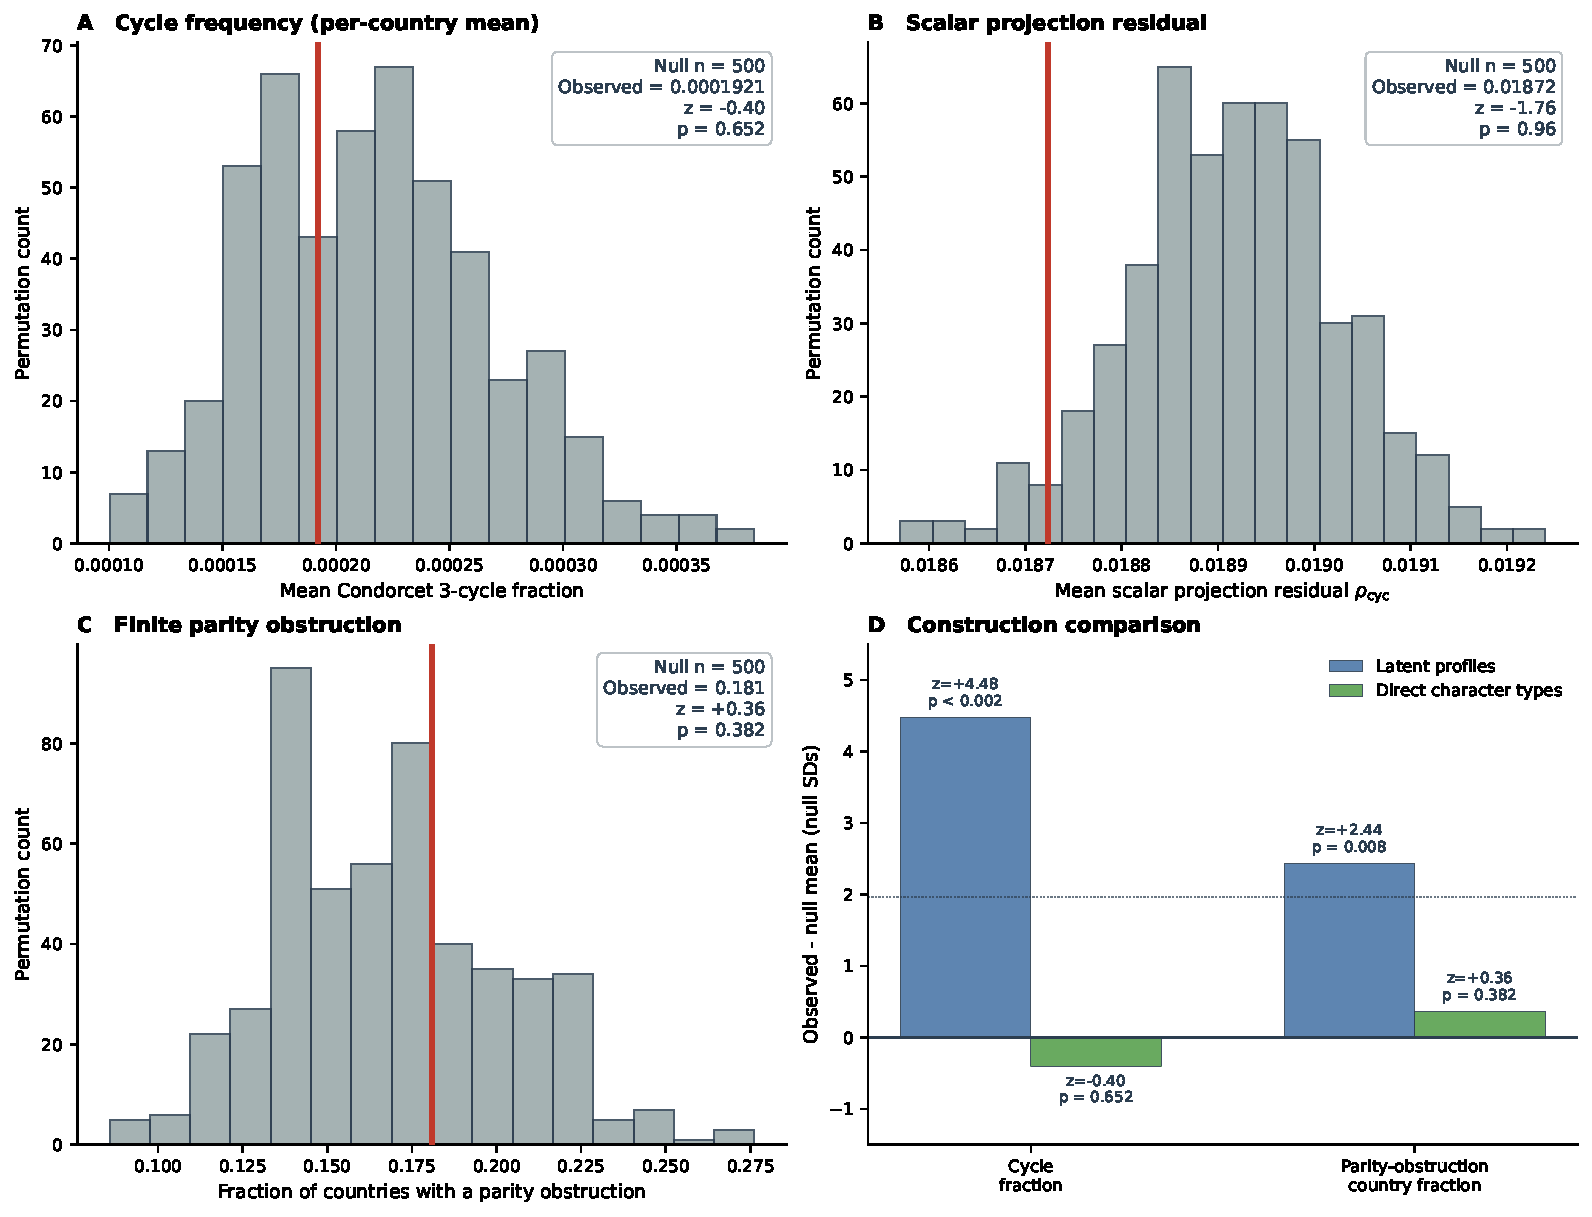
\includegraphics[width=\textwidth]{figures_generated/moral_machine_results.pdf}
\caption{\textbf{Moral Machine diagnostics depend on the alternative construction.} In the direct 20-character construction, country-level moral tournaments in 105 countries contain rare Condorcet cycles and parity obstructions, but their aggregate rates are not elevated above a null that preserves individual preference vectors and country sample sizes while shuffling country labels. The scalar projection residual is also not elevated. A model-based latent moral-profile construction shows larger cycle and parity deviations from its null, indicating that the measured obstruction is partly a property of how moral alternatives are represented.}
\label{fig:mm}
\end{figure}

Figure~\ref{fig:mm} separates the direct and latent Moral Machine conclusions. In the direct 20-character construction, cyclic structure is rare in absolute terms and not elevated above the participant-shuffling null: Figure~\ref{fig:mm}A shows a null-like mean cycle fraction, Figure~\ref{fig:mm}B shows a null-like mean scalar residual, and Figure~\ref{fig:mm}C shows a null-like country fraction with finite parity obstructions. Across the 105 country tournaments we observe 23 Condorcet 3-cycles in total, an average of $0.219$ cycles per country and a mean cycle fraction of $1.92\times 10^{-4}$. The null mean cycle fraction is $2.13\times 10^{-4}$ and the empirical one-sided $p$-value for excess cycles is $0.652$. The mean odd-parity 4-subset fraction is $7.53\times 10^{-4}$, compared with null mean $8.26\times 10^{-4}$ ($p=0.624$). Nineteen of 105 countries (18.1\%) have a non-zero parity-obstruction indicator, close to the null expectation of 16.8\% ($p=0.382$).

The margin-aware scalar residual gives the same conclusion. The mean country-level residual is $\rho_{\mathrm{cyc}}=0.0187$, against a null mean of $0.0189$ ($z=-1.76$, one-sided $p=0.960$ for excess residual). Thus Moral Machine contains exact finite cycles in some country tournaments, and those cycles still obstruct exact scalar representation for those country-level majority relations. But the aggregate cycle, parity, and residual rates do not show excess structure relative to a shuffled-country preference field.

The construction comparison is the substantive result. Figure~\ref{fig:mm}D shows that, in the latent moral-profile construction, cycle and parity diagnostics are elevated relative to the same participant-shuffling logic (cycle fraction $z=4.48$, empirical $p<0.002$; parity-obstruction country fraction $z=2.44$, $p=0.008$). The direct construction therefore calibrates the claim, while the latent construction illustrates the pluralism mechanism: coherent individual moral weights can aggregate into collective relations that no single scalar ordering represents. Moral Machine supports the methodological point rather than the strongest substantive one. Pluralistic systems should measure cycle and residual diagnostics, while recognising that projection loss is defined jointly by the data, the alternative space, and the aggregation map.

\section{Pluralistic, Condorcet-aware alignment}
\label{sec:alignment}

The three case studies suggest a constructive design principle for LLM alignment rather than a blanket impossibility verdict. Scalar reward learning is the wrong default to abandon: it captures the dominant component of human-feedback edge flows almost everywhere, and in PRISM it captures roughly $96\%$ of the weighted LLM preference signal at the population level. MultiPref strengthens this point by showing a dense LLM preference-tuning tournament with no aggregate majority cycles at all. But scalar reward learning is also the wrong default to treat as complete, because residual margin structure remains measurable where pairwise data are available.

A natural model class makes the diagnostic operational. Suppose the population edge flow decomposes as $W = \nabla r^\star + W_{\mathrm{cyc}}$. Standard reward modelling implicitly learns the gradient component $\nabla r^\star$ and discards $W_{\mathrm{cyc}}$. A gradient-plus-residual preference model
\begin{equation}
P(y_i \succ y_j \mid x) \;=\; \sigma\!\bigl(R_\theta(x, y_i)-R_\theta(x, y_j) + C_\phi(x, y_i, y_j)\bigr),
\label{eq:cap}
\end{equation}
with $C_\phi$ antisymmetric in $(y_i, y_j)$ and regularised to be small wherever the scalar component already fits, makes both components estimable. The scalar component $R_\theta$ remains the deployable optimisation signal in coherent regions. The residual term $C_\phi$ functions as a governance signal: it flags regions where optimisation should be cautious, conditional, or pluralistic.

One important boundary of the evidence is that we do not train a reward model or run an RLHF/DPO intervention here. The present results establish $\rho_{\mathrm{cyc}}$ as a diagnostic of scalar representation loss in preference data, not yet as a demonstrated predictor of downstream alignment failure. The routing recommendation should therefore be read as a falsifiable design hypothesis: high-residual regions should be tested for reward-model miscalibration, degraded minority-preference satisfaction, or larger post-training evaluation loss under scalar objectives.

A practical Condorcet-aware alignment pipeline therefore has four elements. First, fit the best scalar component $\nabla r^\star$ on the available preference data and use it as the deployable optimisation signal. Second, compute the cyclic residual $\rho_{\mathrm{cyc}}$ locally, per prompt, per candidate set, or per stratum, and compare aggregate rates against an appropriate null when the support structure permits. Third, in low-residual regions, behave as ordinary RLHF or DPO. Fourth, in high-residual regions, treat the residual as a trigger for testing personalisation, conditional decision rules, multi-objective reward shaping, option preservation, or human deliberation, rather than forcing the residual into the scalar pipeline. The empirical case studies suggest where these regions are likely to appear in practice. In LLM ranking domains analogous to PRISM and MultiPref, the gradient component is often an excellent first approximation, and residuals should be used as calibrated triggers rather than wholesale overrides. Moral Machine adds a caution and an opportunity: the same underlying choices can yield different obstruction profiles under different alternative constructions, so alignment systems should document the representation over which pluralism is being scalarised.

This division of labour turns Condorcet's paradox from a problem into a diagnostic. The cycle is not the failure mode of an aggregation rule; it is the measurement that tells the system its scalar rule should not be used alone.

\section{Discussion}

The picture that the framework and the three case studies together support is deliberately modest but directly relevant to LLM alignment. Human-feedback data are not chaotic, and scalar reward learning is not refuted. The pooled PRISM tournament is overwhelmingly scalar; MultiPref has a strong transitive model-quality ordering; and the direct Moral Machine character-type construction has rare but null-like country-level cycles. What we show is that the residual left by the best scalar ranking can be structurally meaningful and should be measured rather than assumed away. In PRISM, where preferences are rating-based and dominated by a global model-quality axis, the signal is a weighted cyclic residual that is null-like in cycle count but modestly elevated as a fraction of weighted edge-flow energy. In MultiPref, where prompt-local Condorcet tests are not identifiable and aggregate majority cycles are absent, the signal is calibrated aspect-dependent margin non-additivity. In Moral Machine, the contrast between direct character-type tournaments and latent moral-profile tournaments shows that scalar projection loss is not a property of moral data alone. It is a property of a dataset together with the alternatives and aggregation map used to represent pluralism.

The invariants are complementary rather than redundant. Cycle counts are sensitive to qualitative intransitivity but blind to margin information; the weighted residual is sensitive to non-gradient margin geometry but does not by itself show that the underlying majority orientation is cyclic. The methodological lesson is that both should be reported with support audits and appropriate nulls. A null model is needed for claims about enrichment, prevalence, or cultural amplification; it is not needed for the logical implication that an observed cycle is not exactly representable by a scalar ordering. The PRISM case study shows that cycle counts alone can miss small calibrated residual signals. The MultiPref case study shows the converse caution: non-zero residuals in a cleanly ordered tournament should not be redescribed as Condorcet cyclicity.

The localisation results in PRISM are themselves informative. Stated-preference clusters did not become more scalarisable than the pooled tournament; choice attributes did not show that high value salience independently causes residual mass; and demographic strata showed exploratory but not pre-registered residual heterogeneity. Each of these is, in a different way, a negative result against an oversimple pluralistic story. They prevent the social-choice framing from collapsing into a just-so explanation in which any apparent residual is attributed to value heterogeneity. The robust empirical claim is narrower and more useful: the population edge flow contains non-gradient structure whose source cannot be reduced to any single observed covariate we tested.

These findings have several limitations. The parity invariant in Moral Machine is computed from binary majority tournaments and therefore ignores margin magnitudes; we report a margin-aware scalar residual alongside it, but a unified margin-aware topological invariant remains future work. The direct Moral Machine construction uses 20 character-type alternatives derived from saved versus non-saved character counts; the latent construction uses estimated moral-dimension weights and synthetic profile alternatives. Both are defensible, but neither is representation-free, and the contrast between them is precisely why alternative construction should be reported rather than hidden. The participant-shuffling null does not exhaust all modelling assumptions. The PRISM analysis uses opening-turn ballots only; later within-model A/B turns are excluded because they do not compare different source models. The PRISM subgroup residuals are exploratory and reported with false-discovery-rate control rather than as confirmatory tests. The MultiPref calibrated null preserves pair support and annotation weights but does not model prompt-level dependence among annotations; because no prompt group contains a full three-model agenda, MultiPref still cannot support prompt-local Condorcet claims. We also do not test whether $\rho_{\mathrm{cyc}}$ predicts concrete trained-model outcomes, such as reward-model calibration error, minority-preference loss, or RLHF degradation. The non-orientability claim is operational throughout: we do not assert literal manifold non-orientability, and a full topological reconstruction of an explicit cycle complex remains a future validation step.

The constructive implication for alignment practice does not depend on resolving these limitations. Whether the residual mass in PRISM ultimately reflects pluralistic values, context-dependent quality, or some other source, it is a measurable feature ignored by reward models that treat scalar projection as complete. Treating the residual as a governance signal turns a structural feature of preference aggregation into an operational guide. The scalar reward continues to be the workhorse; the cyclic residual tells the system when the workhorse is being asked to do something it cannot.


\bibliographystyle{naturemag}
\begin{thebibliography}{99}\setlength{\itemsep}{1pt}

\bibitem{ouyang2022} Ouyang, L.\ \emph{et al.} Training language models to follow instructions with human feedback. \emph{Adv.\ Neural Inf.\ Process.\ Syst.}\ \textbf{35}, 27730--27744 (2022).

\bibitem{stiennon2020} Stiennon, N.\ \emph{et al.} Learning to summarize with human feedback. \emph{Adv.\ Neural Inf.\ Process.\ Syst.}\ \textbf{33}, 3008--3021 (2020).

\bibitem{rafailov2023} Rafailov, R.\ \emph{et al.} Direct preference optimization: your language model is secretly a reward model. \emph{Adv.\ Neural Inf.\ Process.\ Syst.}\ \textbf{36} (2023).

\bibitem{bai2022} Bai, Y.\ \emph{et al.} Constitutional AI: harmlessness from AI feedback. Preprint at \url{https://arxiv.org/abs/2212.08073} (2022).

\bibitem{arrow1951} Arrow, K.\ J.\ \emph{Social Choice and Individual Values} (Wiley, 1951).

\bibitem{sen1970} Sen, A.\ K. The impossibility of a Paretian liberal. \emph{J.\ Polit.\ Econ.}\ \textbf{78}, 152--157 (1970).

\bibitem{berlin1969} Berlin, I. \emph{Four Essays on Liberty} (Oxford Univ.\ Press, 1969).

\bibitem{raz1986} Raz, J. \emph{The Morality of Freedom} (Clarendon Press, 1986).

\bibitem{black1948} Black, D. On the rationale of group decision-making. \emph{J.\ Polit.\ Econ.}\ \textbf{56}, 23--34 (1948).

\bibitem{plott1967} Plott, C.\ R. A notion of equilibrium and its possibility under majority rule. \emph{Am.\ Econ.\ Rev.}\ \textbf{57}, 787--806 (1967).

\bibitem{mckelvey1976} McKelvey, R.\ D. Intransitivities in multidimensional voting models and some implications for agenda control. \emph{J.\ Econ.\ Theory} \textbf{12}, 472--482 (1976).

\bibitem{chichilnisky1980} Chichilnisky, G. Social choice and the topology of spaces of preferences. \emph{Adv.\ Math.}\ \textbf{37}, 165--176 (1980).

\bibitem{chichilnisky1983} Chichilnisky, G.\ \& Heal, G.\ M. Necessary and sufficient conditions for a resolution of the social choice paradox. \emph{J.\ Econ.\ Theory} \textbf{31}, 68--87 (1983).

\bibitem{baryshnikov1993} Baryshnikov, Y.\ M. Unifying impossibility theorems: a topological approach. \emph{Adv.\ Appl.\ Math.}\ \textbf{14}, 404--415 (1993).

\bibitem{livson2026} Livson, M.\ \emph{et al.} Condorcet's paradox as non-orientability. Preprint (2026).

\bibitem{jiang2011} Jiang, X., Lim, L.-H., Yao, Y.\ \& Ye, Y. Statistical ranking and combinatorial Hodge theory. \emph{Math.\ Program.}\ \textbf{127}, 203--244 (2011).

\bibitem{bradley1952} Bradley, R.\ A.\ \& Terry, M.\ E. Rank analysis of incomplete block designs: I. The method of paired comparisons. \emph{Biometrika} \textbf{39}, 324--345 (1952).

\bibitem{awad2018} Awad, E.\ \emph{et al.} The Moral Machine experiment. \emph{Nature} \textbf{563}, 59--64 (2018).

\bibitem{noothigattu2018} Noothigattu, R.\ \emph{et al.} A voting-based system for ethical decision making. In \emph{Proc.\ AAAI Conf.\ Artif.\ Intell.}\ \textbf{32} (2018).

\bibitem{kim2018moral} Kim, R.\ \emph{et al.} A computational model of commonsense moral decision making. Preprint at \url{https://arxiv.org/abs/1801.04346} (2018).

\bibitem{kirk2024} Kirk, H.\ R.\ \emph{et al.} The PRISM alignment project: what participatory, representative and individualised human feedback reveals about the subjective and multicultural alignment of large language models. Preprint at \url{https://arxiv.org/abs/2404.16019} (2024).

\bibitem{miranda2025} Miranda, L.\ J.\ V.\ \emph{et al.} Hybrid preferences: learning to route instances for human vs.\ AI feedback. Preprint at \url{https://arxiv.org/abs/2410.19133} (2025).

\bibitem{mishra2023} Mishra, A. AI alignment and social choice: fundamental limitations and policy implications. Preprint at \url{https://arxiv.org/abs/2310.16048} (2023).

\bibitem{conitzer2024} Conitzer, V.\ \emph{et al.} Social choice should guide AI alignment in dealing with diverse human feedback. In \emph{Proc.\ Int.\ Conf.\ Mach.\ Learn.}\ (2024).

\bibitem{edelsbrunner2010} Edelsbrunner, H.\ \& Harer, J.\ L.\ \emph{Computational Topology: An Introduction} (Amer.\ Math.\ Soc., 2010).

\bibitem{benjamini1995} Benjamini, Y.\ \& Hochberg, Y. Controlling the false discovery rate: a practical and powerful approach to multiple testing. \emph{J.\ R.\ Stat.\ Soc.\ B} \textbf{57}, 289--300 (1995).

\bibitem{plank2014} Plank, B., Hovy, D.\ \& S\o{}gaard, A. Linguistically debatable or just plain wrong? In \emph{Proc.\ Annu.\ Meeting Assoc.\ Comput.\ Linguist.}\ 507--511 (2014).

\bibitem{pavlick2019} Pavlick, E.\ \& Kwiatkowski, T. Inherent disagreements in human textual inferences. \emph{Trans.\ Assoc.\ Comput.\ Linguist.}\ \textbf{7}, 677--694 (2019).

\bibitem{dawid1979} Dawid, A.\ P.\ \& Skene, A.\ M. Maximum likelihood estimation of observer error-rates using the EM algorithm. \emph{J.\ R.\ Stat.\ Soc.\ C} \textbf{28}, 20--28 (1979).

\bibitem{zhu2023} Zhu, Y., Jiao, J.\ \& Jordan, M.\ I. Principled RLHF from pairwise or K-wise comparisons. In \emph{Proc.\ Int.\ Conf.\ Mach.\ Learn.}\ (2023).

\bibitem{gibbard1973} Gibbard, A. Manipulation of voting schemes: a general result. \emph{Econometrica} \textbf{41}, 587--601 (1973).

\bibitem{satterthwaite1975} Satterthwaite, M.\ A. Strategy-proofness and Arrow's conditions. \emph{J.\ Econ.\ Theory} \textbf{10}, 187--217 (1975).

\bibitem{kahneman1982} Kahneman, D., Slovic, P.\ \& Tversky, A.\ \emph{Judgment Under Uncertainty: Heuristics and Biases} (Cambridge Univ.\ Press, 1982).

\bibitem{simonson2008} Simonson, I. Constructed and inherent preferences. \emph{J.\ Consum.\ Psychol.}\ \textbf{18}, 155--169 (2008).

\bibitem{coste2023} Coste, T.\ \emph{et al.} Reward model ensembles help mitigate overoptimization. Preprint at \url{https://arxiv.org/abs/2310.02743} (2023).

\bibitem{eisenstein2023} Eisenstein, J.\ \emph{et al.} Helping or herding? Reward model ensembles mitigate but do not eliminate reward hacking. Preprint at \url{https://arxiv.org/abs/2312.09244} (2023).

\bibitem{thurstone1927} Thurstone, L.\ L. A law of comparative judgment. \emph{Psychol.\ Rev.}\ \textbf{34}, 273--286 (1927).

\bibitem{chichilnisky1991} Chichilnisky, G. Social choice and the closed convergence topology. \emph{Soc.\ Choice Welf.}\ \textbf{8}, 307--317 (1991).

\end{thebibliography}

\clearpage

\section*{Methods}

\subsection*{PRISM: data and opening-turn extraction}

We use the public PRISM release on Hugging Face (\texttt{HannahRoseKirk/prism-alignment})\cite{kirk2024}. The conversations split stores each conversation as a nested history. Each conversation is retained if turn 0 contains at least three scored model responses with non-null model names. Of the 1,500 surveyed participants, 1,396 progressed to conversations; the canonical analysis uses 7,828 opening-turn ballots after applying score-threshold settings and excluding ties.

\subsection*{PRISM: pairwise comparisons and user-weighted aggregation}

For each opening turn $c$ by user $u$ presenting models in subset $S_{uc}$ with scores $s_{uc}(\cdot)\in\{1,\ldots,100\}$, and for score-difference threshold $\delta\geq 0$, the induced pairwise comparison is
\[
Y^{(\delta)}_{uc,ij} \;=\;
\begin{cases}
+1, & s_{uc}(i)-s_{uc}(j)>\delta,\\
-1, & s_{uc}(j)-s_{uc}(i)>\delta,\\
0,  & |s_{uc}(i)-s_{uc}(j)|\leq\delta.
\end{cases}
\]
Canonical setting: $\delta=5$. We aggregate first within users by averaging non-tied comparisons across that user's conversations involving the same model pair, then across users equally. Edges with fewer than $n_{\min}=25$ contributing users are excluded. The canonical orientation threshold is $\tau=0$. The resulting matrix $W$ is skew-symmetric, $W_{ij}=-W_{ji}$, and support weights $\omega_{ij}$ are the per-edge user counts.

\subsection*{PRISM: cycle rate and Hodge residual}

The cycle rate is the proportion of eligible triples $(i,j,k)$ for which $W_{ij}>\tau$, $W_{jk}>\tau$, $W_{ki}>\tau$, or the reverse-oriented analogue holds, among all triples with all three edges present. The cyclic residual mass $\rho_{\mathrm{cyc}}(W)$ is computed by solving the weighted least-squares problem in Equation~\eqref{eq:rstar} for $r^\star$ and evaluating Equation~\eqref{eq:rho}. The additive degree of freedom in $r$ is fixed by centring scores to mean zero. Undefined statistics, such as cycle rates on subgraphs with no eligible triples, are reported as undefined rather than zero.

For PRISM threshold sensitivity, we sweep $\delta\in\{0,2,5,10\}$, $n_{\min}\in\{10,25,50,100\}$, and $\tau\in\{0,0.05,0.10\}$. The orientation threshold $\tau$ is used only for binary cycle counting; the Hodge residual uses the signed margins and edge supports directly. The transitive-null analysis reported in the main text uses the canonical setting $\delta=5$, $n_{\min}=25$, and $\tau=0$.

\subsection*{PRISM: fitted transitive null}

For each observed tournament, we fit a Bradley--Terry-style scalar edge model\cite{bradley1952} by weighted least squares on the empirical margins, holding the observed edge supports and support weights fixed. We then simulate $B=5{,}000$ synthetic tournaments under this transitive data-generating process with the same supports, and recompute cycle rate and $\rho_{\mathrm{cyc}}$ on each simulation. Empirical Monte Carlo $p$-values are $(1+\#\{T_b\geq T_{\mathrm{obs}}\})/(1+B)$. This null tests how much cyclic structure a transitive process would produce under finite-sample noise with the same supports; it is not required for the structural cycle-obstruction claim (Proposition~\ref{prop:cycle}).

\subsection*{PRISM: stated-preference clusters and demographic strata}

Stated-preference vectors over creativity, diversity, factuality, fluency, helpfulness, personalisation, safety, and values are standardised before clustering. Demographic strata use English proficiency, marital status, age, education, and gender. For each stratification, we recompute the user-weighted edge flow within stratum, apply the same edge-support threshold $n_{\min}=25$, and run the fitted transitive null. Multiple-comparison correction uses the Benjamini--Hochberg false-discovery-rate procedure\cite{benjamini1995} rather than Bonferroni, since strata are correlated and not pre-registered as primary hypotheses; results are reported as exploratory group-level edge-flow properties rather than confirmatory tests or causal claims.

\subsection*{Choice attributes}

PRISM's choice attributes are winner-conditioned: they record why the highest-rated model was preferred relative to the other opening-turn models. We use them as filters defining high- and low-attribute subsets and as edge-level metadata, but do not infer per-model factuality, safety, or helpfulness scores for losing models from these fields. High-attribute subsets are compared against matched transitive nulls with the same supports to control for changes in edge support.

\subsection*{MultiPref: data and flattening}

We use the public MultiPref release (\texttt{allenai/multipref})\cite{miranda2025}. The default training split contains 10,461 pairwise response-comparison rows. Each row has a stable \texttt{prompt\_id}, literal prompt text, source-model identifiers \texttt{model\_a} and \texttt{model\_b}, completions, and nested lists of normal-worker and expert-worker annotation dictionaries. We flatten normal and expert annotations into one row per human annotation, producing 31,934 annotation rows. Each annotation provides overall, helpfulness, truthfulness, and harmlessness preference labels. Labels are mapped to signed weighted contributions relative to the row-local A/B roles: \texttt{A-is-clearly-better} and \texttt{B-is-clearly-better} have weight 1, \texttt{A-is-slightly-better} and \texttt{B-is-slightly-better} have weight 0.5, and ties have weight 0. A/B labels are never treated as global alternatives; they are mapped to the stable source models in \texttt{model\_a} and \texttt{model\_b}.

\subsection*{MultiPref: prompt support and global tournament}

For each prompt grouping column (\texttt{prompt\_id} and, as a sensitivity check, literal prompt text), we collapse repeated annotations to unique unordered source-model pairs. For each group we record the number of distinct models, observed model-pair edges, possible model-pair edges, and fully supported three-model triangles. A prompt-local Condorcet test is identifiable only when at least one model triple has all three unordered pair edges observed. No MultiPref prompt group satisfies this condition under either grouping.

For the global source-model analysis, we aggregate across prompts to a six-model tournament. For each aspect and annotation group (pooled, normal, expert), we compute weighted pairwise margins, majority cycle counts among the 20 fully supported triples, and $\rho_{\mathrm{cyc}}$ by solving Equation~\eqref{eq:rstar}. Same-model comparisons are excluded from support audits and global model-pair summaries. To calibrate the global residuals, we fit the closest bounded additive margin flow $m_{ij}=r_i-r_j$ by weighted least squares on the observed model-pair support. The null then resamples non-tie signs on each observed edge with $\mathbb{E}[\mathrm{sign}_{ij}]=m_{ij}$ while preserving the number and weights of annotations on that edge. We use $5{,}000$ simulations per group-aspect cell and report one-sided empirical $p$-values with Benjamini--Hochberg correction across the 12 MultiPref residual tests.

\subsection*{Moral Machine: data, preference estimation, and tournament construction}

We use the public Moral Machine release (\texttt{https://osf.io/3hvt2/})\cite{awad2018}. Each scenario contributes two outcome-side rows, one saved and one not saved. For each retained respondent, we construct a signed preference vector over the 20 canonical character types by summing character counts on saved rows and subtracting character counts on non-saved rows, then dividing by the number of valid saved-side scenarios. Respondents with fewer than eight valid scenarios are excluded. This row-wise construction preserves the paired contrast while avoiding assumptions about file ordering or chunk boundaries. It retains 1,851,181 respondents. For each country with at least 200 retained respondents, the pairwise majority across respondent character-type scores defines a tournament on the 20 character-type alternatives; 105 country tournaments qualify. For the margin analysis, the edge margin $W_{cd}$ is $(n_{c>d}-n_{d>c})/(n_{c>d}+n_{d>c})$, with support $n_{c>d}+n_{d>c}$ after excluding respondent-level ties on that pair.

For the latent moral-profile comparison, following prior Moral Machine modelling that treats choices as trade-offs over moral dimensions\cite{awad2018,noothigattu2018,kim2018moral}, we estimate respondent-level signed weights over moral dimensions from the scenario attributes, retaining respondents with at least eight usable scenarios and at least four covered dimensions. A finite set of synthetic moral profiles is represented by vectors $x_m\in\{-1,+1\}^{d}$ over the retained moral dimensions. Respondent $i$ assigns profile $m$ the linear utility $u_i(m)=\langle\beta_i,x_m\rangle$. For each country with sufficient retained respondents, pairwise majority comparisons over these profile utilities define a country tournament. We apply the same finite cycle, parity, and participant-shuffling logic to this model-based profile tournament. This comparison is used to test how the measured obstruction changes when the alternative space is moral-profile based rather than character-type based.

\subsection*{Moral Machine: finite cycle and parity invariants}

For each country tournament we compute three finite orientation invariants and one margin-aware residual. The cycle fraction is the proportion of the $\binom{20}{3}=1{,}140$ triples whose restriction of $T$ is a Condorcet cycle (all three vertices have in-degree one). The odd-parity 4-subset fraction is the proportion of the $\binom{20}{4}=4{,}845$ 4-subsets whose cycle-indicator parity, summed across the four triangular faces modulo $2$, is odd. The parity-obstruction indicator is $1$ if at least one 4-subset has odd parity. We also compute $\rho_{\mathrm{cyc}}$ from the signed country margins and pair supports by solving Equation~\eqref{eq:rstar}. The finite parity computations scale as $O(K^{4})$ per tournament. These finite statistics are motivated by the simplicial construction of Livson \emph{et al.}\cite{livson2026} but do not by themselves establish literal manifold non-orientability.

\subsection*{Moral Machine: participant-shuffling null}

To distinguish country structure from finite-sample noise and global respondent-level preference heterogeneity, we use a permutation null with $n=500$ permutations. Each permutation shuffles country labels across retained respondents while preserving each respondent's signed character-type vector and each country's group size. For each permutation we recompute the country-level tournaments, signed margins, pair supports, three finite invariants, and scalar residual. Standardised deviations are $z=(\text{obs}-\text{null mean})/\text{null SD}$. Empirical $p$-values are $(1+\#\{T_b\geq T_{\mathrm{obs}}\})/(1+n)$ for the per-country mean cycle fraction, per-country mean odd-parity fraction, country fraction with non-zero parity-obstruction indicator, and mean country-level $\rho_{\mathrm{cyc}}$.

\subsection*{Data and code availability}

The Moral Machine dataset is publicly available at \texttt{https://osf.io/3hvt2/}\cite{awad2018}. The PRISM alignment dataset is publicly available at \texttt{https://huggingface.co/datasets/HannahRoseKirk/prism-alignment}\cite{kirk2024}. MultiPref is publicly available at \texttt{https://huggingface.co/datasets/allenai/multipref}\cite{miranda2025}. Reproduction code in Python, including PRISM parsing, MultiPref flattening and support audits, edge-flow construction, cycle and Hodge residual computation, transitive-null simulation where used, the participant-shuffling null for Moral Machine, and figure generation, will be released in a public repository upon publication.

\end{document}
